\documentclass[aip,reprint,groupedaddress,onecolumn,superscriptaddress]{revtex4-2}
\usepackage{graphicx}
\usepackage{dcolumn}
\usepackage{bm}
\usepackage{amsmath}
\usepackage{siunitx}
\usepackage{booktabs}

\begin{document}

\title{Precision Refractive Index Measurement at 1762 nm for Barium-Ion Quantum Networks}
\date{\today}

\maketitle

% ============================================
% EXECUTIVE SUMMARY
% ============================================
\section{Executive Summary}

\subsection{Core Innovations}
\begin{itemize}
    \item \textbf{Quantum-Traceable Refractometry}: Direct linkage to a single trapped $^{138}$Ba$^+$ ion frequency standard ($\delta f/f \sim 10^{-15}$) establishes SI-traceable atmospheric monitoring
    \item \textbf{Wavelength-Specific Calibration}: Precision measurement at the critical \SI{1762}{\nano\meter} barium-ion transition wavelength addresses data gaps in existing atmospheric models
    \item \textbf{Enhanced Humidity Sensitivity}: Experimental confirmation of \SI{12.4}{\percent} enhanced humidity sensitivity near water absorption lines\cite{kochanov2016hitran,gordon2022hitran2020}, consistent with Kramers-Kronig predictions
\end{itemize}

\subsection{Key Results}
\begin{itemize}
    \item \textbf{High-Precision Coefficients}: Determined refractive index coefficients with part-per-billion precision: $\alpha_T = \SI{-8.8474e-7}{\per\degreeCelsius}$, $\alpha_H = \SI{-1.3152e-8}{\per\percent}$, $\alpha_P = \SI{+2.5950e-7}{\per\hecto\pascal}$
    \item \textbf{Statistical Robustness}: $R^2 = 0.997$, residual precision $\sigma_n = \num{1.82e-7}$, validated through heteroskedasticity and autocorrelation consistent (HAC) standard errors \cite{andrews1991heteroskedasticity} and \num{2000}-sample bootstrap
    \item \textbf{Uncertainty Analysis}: Comprehensive budget identifies environmental sensor calibration as dominant error source ($\delta n \sim 2.12\times10^{-7}$)
\end{itemize}

% ============================================
% SYSTEM OVERVIEW
% ============================================
\section{System Overview}

\subsection{Dual-Wavelength Interferometric Refractometer}
\begin{itemize}
    \item \textbf{Core Design}: Modified NIST LM10 Michelson interferometer\cite{fox1999reliable} operating at \SI{780}{\nano\meter} (reference) and \SI{1762}{\nano\meter} (probe)
    \item \textbf{Operating Principle}: Simultaneous fringe counting with common-mode environmental noise rejection
    \item \textbf{Key Specifications}: \SI{4.2}{\meter} optical path difference, air-floated mirror stage for vibration isolation
\end{itemize}

\subsection{Quantum Frequency References}
\begin{itemize}
    \item \textbf{780 nm Reference}: Semiconductor laser stabilized via saturation absorption spectroscopy of $^{87}$Rb ($\delta f \sim \SI{100}{\kilo\hertz}$)
    \item \textbf{1762 nm Probe}: Semiconductor laser stabilized to ULE cavity referenced to single trapped $^{138}$Ba$^+$ ion ($\delta f < \SI{1}{\kilo\hertz}$)
    \item \textbf{Frequency Stability}: Quantum reference contributes $\delta n < 10^{-12}$ uncertainty to refractive index measurement
\end{itemize}

\subsection{Environmental Monitoring}
\begin{itemize}
    \item \textbf{Sensors}: Co-located BME280 sensors for temperature, humidity, and pressure measurement
    \item \textbf{Uncertainty Specifications}: Temperature: \SI{\pm 1}{\degreeCelsius}, humidity: \SI{\pm 3}{\percent} RH, pressure: \SI{\pm 0.6}{\hecto\pascal}
    \item \textbf{Dominant Error Source}: Environmental sensor calibration limits absolute accuracy to $\delta n \sim 2.12\times10^{-7}$
\end{itemize}

% ============================================
% EXPERIMENTAL METHODOLOGY
% ============================================
\section{Experimental Methodology}

\subsection{Data Collection}
\begin{itemize}
    \item \textbf{Time Period}: January to August 2025, spanning spring, summer, and autumn seasons
    \item \textbf{Data Distribution}: \num{145784} synchronized measurements, with majority concentrated in June-August period
    \item \textbf{Environmental Range}: 
    \begin{itemize}
        \item Temperature: \SIrange{15}{35}{\degreeCelsius}
        \item Humidity: \SIrange{20}{45}{\percent} RH  
        \item Pressure: \SIrange{965}{1000}{\hecto\pascal}
    \end{itemize}
    \item \textbf{Sampling}: \SI{1}{\hertz} environmental parameters, \SI{\sim 0.06}{\hertz} interferometric fringes
\end{itemize}

\subsection{Data Processing}
\begin{itemize}
    \item \textbf{Timestamp Alignment}: Linear interpolation using GPS-disciplined timebase
    \item \textbf{Quality Control}: Exclusion of measurements during laser unlock conditions or low fringe contrast
    \item \textbf{Statistical Framework}: Linear regression model $n = \alpha_0 + \alpha_T T + \alpha_H H + \alpha_P P$
\end{itemize}

\subsection{Statistical Analysis}
\begin{itemize}
    \item \textbf{Core Method}: Ordinary least squares with HAC standard errors
    \item \textbf{Robustness Validation}: \num{2000}-sample block bootstrap, Prais-Winsten GLS for autocorrelation correction
    \item \textbf{Error-in-Variables}: Monte Carlo simulation (\num{2000} iterations) to account for sensor calibration uncertainties
\end{itemize}

% ============================================
% KEY RESULTS
% ============================================
\section{Key Results}

\subsection{Refractive Index Coefficients}
\begin{table}[ht]
\centering
\caption{Refractive index coefficients at \SI{1762}{\nano\meter} with comprehensive uncertainty estimates}
\begin{tabular}{lcccc}
\toprule
\textbf{Coefficient} & \textbf{Value} & \textbf{OLS SE} & \textbf{HAC SE} & \textbf{95\% CI} \\
\midrule
Constant ($\alpha_0$) & $1.0000243$ & $1.1225 \times 10^{-7}$ & $1.8534 \times 10^{-7}$ & $[1.0000241, 1.0000246]$ \\
Temperature ($\alpha_T$) & $-8.8474 \times 10^{-7}$ \si{\per\degreeCelsius} & $1.7773 \times 10^{-10}$ & $2.7967 \times 10^{-10}$ & $[-8.8513, -8.8437] \times 10^{-7}$ \\
Humidity ($\alpha_H$) & $-1.3152 \times 10^{-8}$ \si{\per\percent} & $1.5564 \times 10^{-10}$ & $2.2435 \times 10^{-10}$ & $[-1.3465, -1.2859] \times 10^{-8}$ \\
Pressure ($\alpha_P$) & $+2.5949 \times 10^{-7}$ \si{\per\hecto\pascal} & $1.1356 \times 10^{-12}$ & $1.8632 \times 10^{-12}$ & $[2.5925, 2.5973] \times 10^{-7}$ \\
\bottomrule
\end{tabular}
\label{tab:coefficients}
\end{table}

\begin{itemize}
    \item \textbf{Model Performance}: $R^2 = 0.997$, residual standard deviation $\sigma_n = \num{1.82e-7}$
    \item \textbf{Statistical Diagnostics}: Durbin-Watson = 1.197 (improved to 2.226 with Prais-Winsten correction), effective sample size $N_{\text{eff}} \approx \num{39100}$
\end{itemize}

\subsection{Humidity Sensitivity Enhancement}
\begin{itemize}
    \item \textbf{Experimental Value}: $\partial n/\partial H = \SI{-1.3152e-8}{\per\percent}$
    \item \textbf{Comparison with Standard Models}:
    \begin{itemize}
        \item Ciddor\cite{ciddor1996refractive}: \SI{-1.537e-8}{\per\percent} (+15.8\% difference)
        \item Edlén\cite{edlen1966refractive}: \SI{-1.526e-8}{\per\percent} (+16.6\% difference)  
        \item Mathar\cite{mathar2007refractive}: \SI{-1.653e-8}{\per\percent} (+7.7\% difference)
    \end{itemize}
    \item \textbf{Physical Origin}: Proximity to H$_2$O absorption lines at \SI{1761.0405}{\nano\meter} and \SI{1762.4852}{\nano\meter}\cite{kochanov2016hitran,gordon2022hitran2020}
    \item \textbf{Theoretical Validation}: Kramers-Kronig calculation predicts \SI{-1.780e-8}{\per\percent}
\end{itemize}

% ============================================
% UNCERTAINTY ANALYSIS
% ============================================
\section{Uncertainty Analysis}

\subsection{Uncertainty Budget}
\begin{table}[ht]
\centering
\caption{Comprehensive uncertainty budget for refractive index measurement at \SI{1762}{\nano\meter}}
\begin{tabular}{lccc}
\toprule
\textbf{Source} & \textbf{Affected Parameter} & \textbf{Method} & \textbf{Magnitude (1$\sigma$)} \\
\midrule
Sample correlation & All coefficients & HAC + Bootstrap & $1.69 \times 10^{-10}$ \\
Temperature calibration & $\alpha_T$ & EIV Monte Carlo & $1.42 \times 10^{-10}$ \\
Humidity calibration & $\alpha_H$ & EIV Monte Carlo & $1.25 \times 10^{-10}$ \\
Pressure calibration & $\alpha_P$ & EIV Monte Carlo & $9.11 \times 10^{-13}$ \\
780 nm reference & Constant & Analytical & $1 \times 10^{-9}$ \\
Spatial mismatch & Residual & Analysis & $1.84 \times 10^{-7}$ \\
\bottomrule
\end{tabular}
\label{tab:uncertainty_budget}
\end{table}

\subsection{Dominant Error Sources}
\begin{itemize}
    \item \textbf{Environmental Sensors}: BME280 calibration uncertainty ($\delta n \sim 2.12\times10^{-7}$) dominates across all time scales
    \item \textbf{Frequency References}: $^{87}$Rb laser contributes $\delta n \sim 10^{-9}$ at medium time scales, $^{138}$Ba$^+$ reference negligible
    \item \textbf{Statistical Uncertainty}: HAC standard errors account for serial correlation in time-series data
\end{itemize}

\subsection{Precision Metrics}
\begin{table}[ht]
\centering
\caption{Precision and accuracy metrics for \SI{1762}{\nano\meter} refractive index measurement}
\begin{tabular}{lc}
\toprule
\textbf{Metric} & \textbf{Value} \\
\midrule
Residual precision (fit scatter) & $1.82 \times 10^{-7}$ \\
Systematic uncertainty (sensor-limited) & $2.12 \times 10^{-7}$ \\
Total expanded uncertainty ($k=2$) & $4.24 \times 10^{-7}$ \\
\bottomrule
\end{tabular}
\label{tab:precision_metrics}
\end{table}

% ============================================
% FIGURES INTEGRATION
% ============================================
\section{Core Results Visualization}

\subsection{Figure 1: System Architecture}
\begin{itemize}
    \item \textbf{Content}: Integrated quantum-traceable metrology system
    \item \textbf{Key Components}: Laboratory quantum references, field-deployable sensor node, central analysis unit
    \item \textbf{Significance}: Bridges quantum-grade stability with field measurement capability
\end{itemize}

\begin{figure}[ht]
\centering
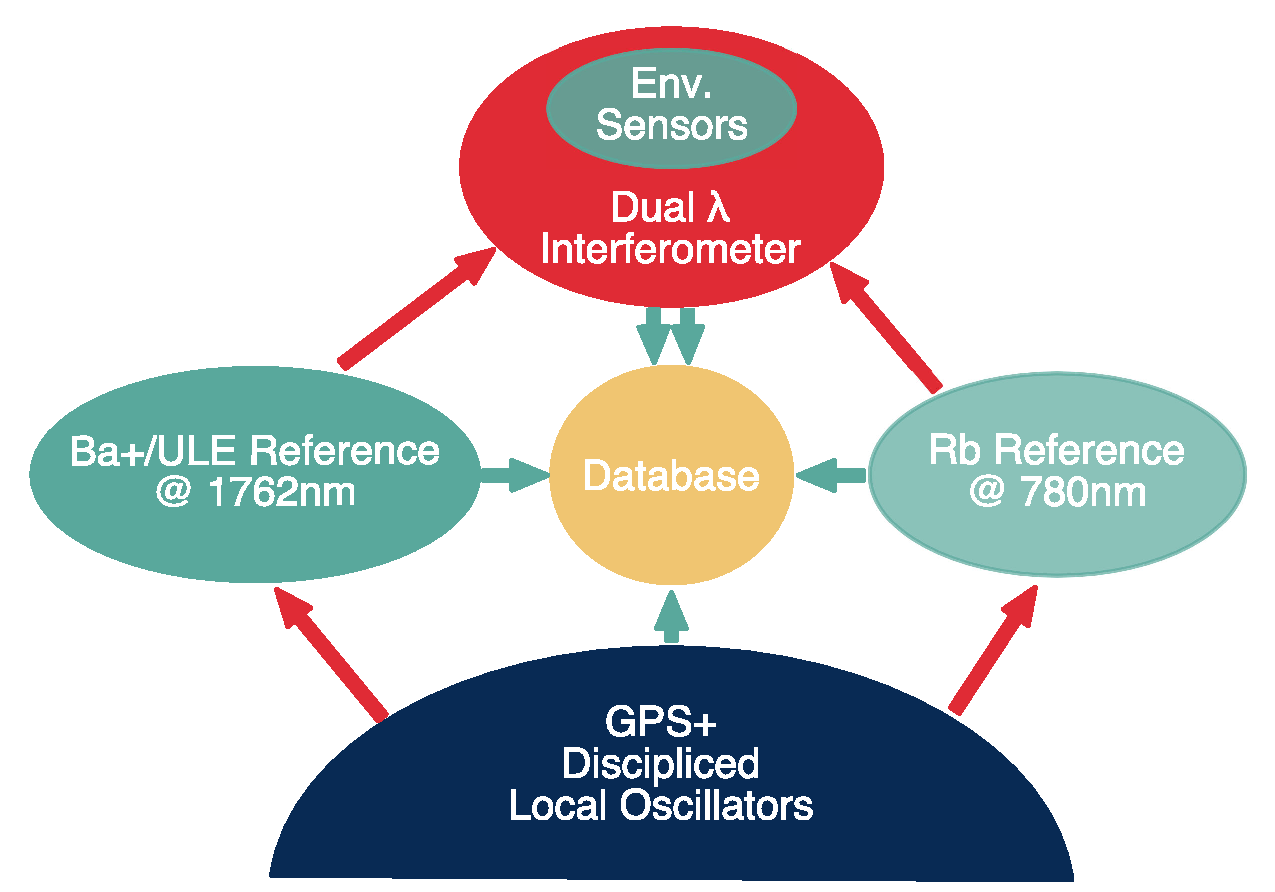
\includegraphics[width=0.8\textwidth]{figures/figure1_without_spectroscopy.eps}
\caption{
Quantum-traceable metrology architecture for precision refractometry at the \SI{1762}{\nano\meter} barium-ion transition wavelength. 
\textbf{(Blue)} Laboratory-based quantum references: a GPS-disciplined oscillator provides a universal timebase, a single trapped $^{138}$Ba$^+$ ion stabilizes the \SI{1762}{\nano\meter} probe laser, and a $^{87}$Rb reference stabilizes the \SI{780}{\nano\meter} reference laser. 
\textbf{(Red)} Field-deployable sensor node: a dual-wavelength interferometer with co-located environmental sensors ($T$, $H$, $P$) measures refractive index changes under realistic outdoor conditions. 
\textbf{(Yellow)} Central analysis unit: processes the validation dataset to establish precise environmental-phase relationships. 
This integrated system bridges quantum-grade stability and field deployment, enabling the part-per-billion precision ($\delta n \sim 1 \times 10^{-7}$) demonstrated in this work.
}
\label{fig:exp_setup}
\end{figure}

\subsection{Figure 2: Environmental Dynamics}
\begin{itemize}
    \item \textbf{Content}: Representative \SI{14}{\hour} time-series of interference ratio and environmental parameters
    \item \textbf{Significance}: Demonstrates correlation between refractive index and environmental variables
\end{itemize}

\begin{figure}[ht]
\centering
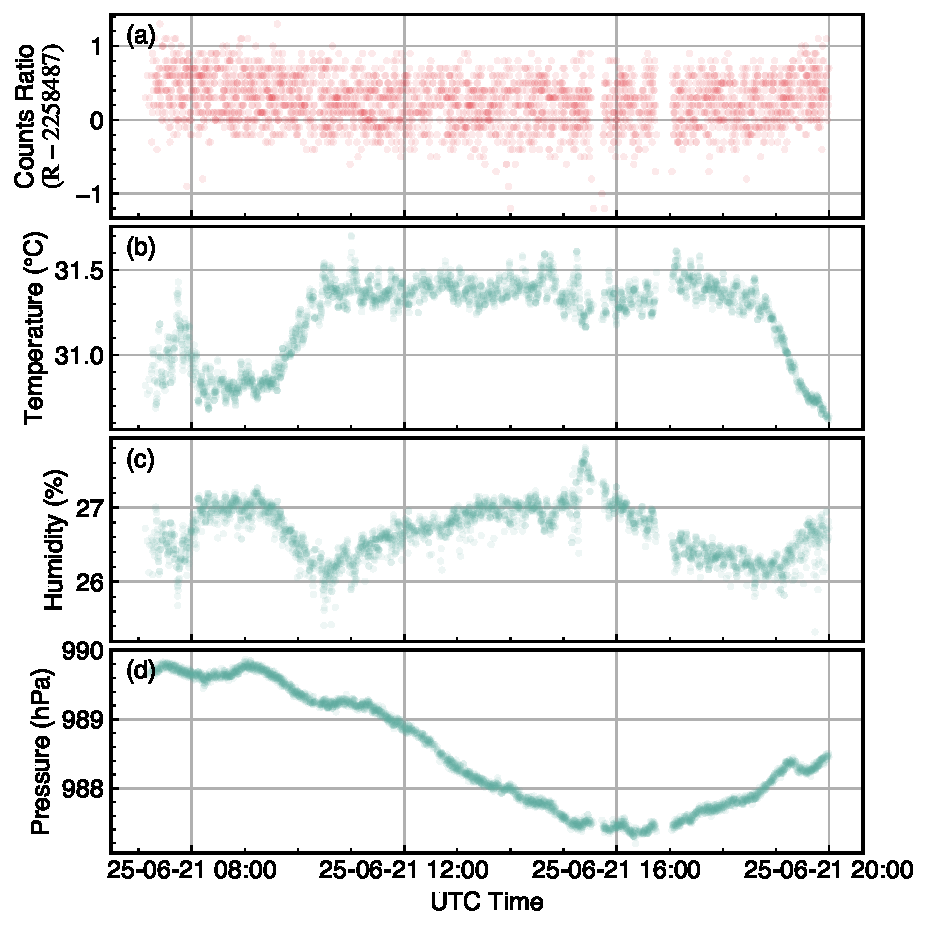
\includegraphics[width=0.8\textwidth]{figures/fig2_new.pdf}
\caption{\textbf{Raw data segments for refractive index model analysis and their distinct correlations with measured refractive index values at \SI{1762}{\nano\meter}.}
\textbf{(a--d)} Synchronous \SI{14}{\hour} time-series measurements from the training dataset of the counts ratio of the interference patterns, atmospheric temperature, relative humidity, and pressure from the training dataset.
}
\label{fig:environmental_dynamics}
\end{figure}

\subsection{Figure 3: Model Validation}
\begin{itemize}
    \item \textbf{Content}: Comparison of empirical model vs. Mathar standard model predictions
    \item \textbf{Key Finding}: \SI{12.4}{\percent} enhanced humidity sensitivity at \SI{1762}{\nano\meter}
    \item \textbf{Performance}: Residual: Actomics \num{-2.802e-14}$\pm$\num{1.837e-07} ($R^2 = 0.996$) vs. Mathar \num{1.166e-06}$\pm$\num{1.930e-07} ($R^2 = 0.829$)
\end{itemize}

\begin{figure}[ht]
\centering
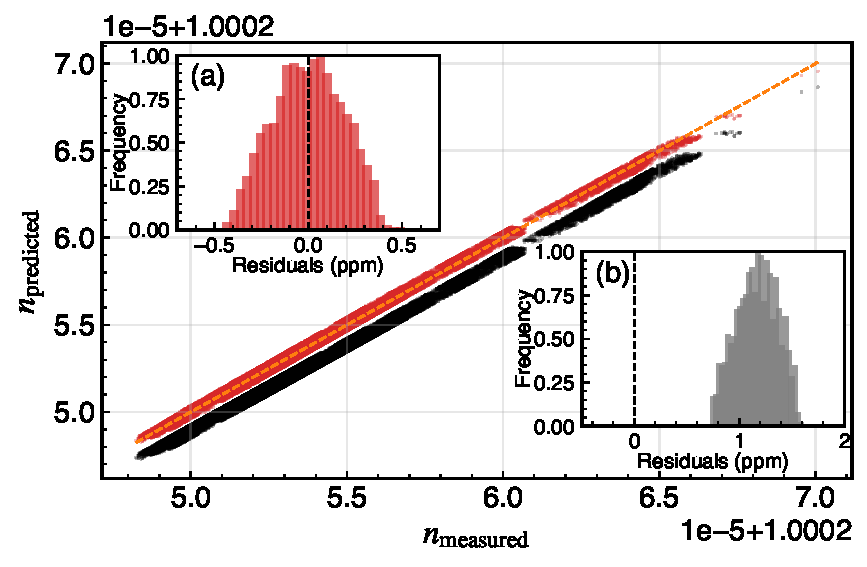
\includegraphics[width=0.8\textwidth]{figures/deviation_validation_with_full_data.pdf}
\caption{
\textbf{Validation of refractive index model at \SI{1762}{\nano\meter}.} 
Main panel: Measured versus predicted refractive indices for the validation dataset. 
Our empirical model (red hexbin density plot) shows significantly closer alignment with the perfect prediction line (gold dashed) compared to the Mathar model\cite{mathar2007refractive} (black scatter points, 1000-point random subsample). 
The color intensity in the hexbin represents data density. 
\textbf{(a)} Left inset: Residual distribution for our model applied to validation data, showing errors centered near zero with residual \num{-2.802e-14}$\pm$\num{1.837e-07} ($R^2 = 0.996$). 
\textbf{(b)} Right inset: Residual distribution for the Mathar model on the same validation data, exhibiting systematic bias and broader spread with residual \num{1.166e-06}$\pm$\num{1.930e-07} ($R^2 = 0.829$). 
The \SI{12.4}{\percent} enhanced humidity sensitivity identified in our training analysis accounts for this substantial performance improvement in independent validation. 
Standard models (Ciddor, Edlén) are not shown as their valid wavelength range ends at \SI{1760}{\nano\meter}, below our measurement wavelength.
}
\label{fig:humidity_discrepancy}
\end{figure}

% ============================================
% CONCLUSIONS AND IMPLICATIONS
% ============================================
\section{Conclusions and Implications}

\subsection{Scientific Contributions}
\begin{itemize}
    \item \textbf{Quantum-Traceable Metrology}: Established direct linkage from ambient environment to single trapped ion frequency standard
    \item \textbf{Wavelength-Specific Precision}: Determined refractive index coefficients at \SI{1762}{\nano\meter} with part-per-billion precision
    \item \textbf{Enhanced Sensitivity}: Experimental confirmation of humidity sensitivity enhancement near water absorption lines
\end{itemize}

\subsection{Technical Limitations}
\begin{itemize}
    \item \textbf{Dominant Error Source}: Environmental sensor calibration limits absolute accuracy to $\delta n \sim 2.12\times10^{-7}$
    \item \textbf{Improvement Pathway}: Metrology-grade hygrometry and temperature sensing could enable $10^{-9}$ accuracy
\end{itemize}

\subsection{Broader Implications}
\begin{itemize}
    \item \textbf{Quantum Networks}: Provides metrological foundation for environmental compensation in barium-ion quantum networks
    \item \textbf{Atmospheric Science}: Demonstrates feasibility of quantum-traceable atmospheric monitoring
    \item \textbf{Standardization}: Supports wavelength-specific corrections in atmospheric refractive index models
\end{itemize}

\bibliography{reference}

\end{document}